\chapter{L'azienda}
\label{cap:lazienda}


\section{\azienda}

\subsection{Descrizione}
L'azienda {\azienda}, fondata nel 1984, offre servizi di consulenza e sviluppo di software. 
Si è distinta nell'ideazione, costruzione e implementazione di strumenti software per oltre 2500 imprese, 
molte delle quali all'estero. \\
Una delle sue qualità distintive è l'attenzione verso i clienti, 
con vari uffici in regioni come Veneto, Lombardia, Emilia-Romagna, Friuli-Venezia Giulia, Toscana, Puglia e Campania, 
impiegando oltre 600 professionisti. \\
La sede centrale per la ricerca e sviluppo (CSV) si trova a Grisignano di Zocco (VI) e ospita più di 200 collaboratori. 
Qui, gruppi di sviluppatori 
e tecnici lavorano insieme per assicurare servizi affidabili e soluzioni software su misura. 
\newpage

\subsection{Organizzazione dell'azienza e i suoi prodotti}
{\azienda} è suddivisa in \textit{Business Unit} (BU), una parte di un'azienda che opera in modo autonomo o semi-autonomo, 
con la propria visione, \textit{mission}, obiettivi e strategie. Essa ha una propria \textit{leadership} e una struttura 
organizzativa separata, ed è responsabile del proprio profitto e perdite. \\
Le BU possono focalizzarsi su 
specifici mercati geografici, gruppi di clienti o linee di prodotti, permettendo all'azienda di essere 
più agile e rispondere meglio alle esigenze del mercato e dei clienti.\\
In {\azienda} BU sono 11 e sono rappresentate in figura \ref{fig:organizzazione-azienda}.\\

\begin{figure}[!h] 
  \centering 
  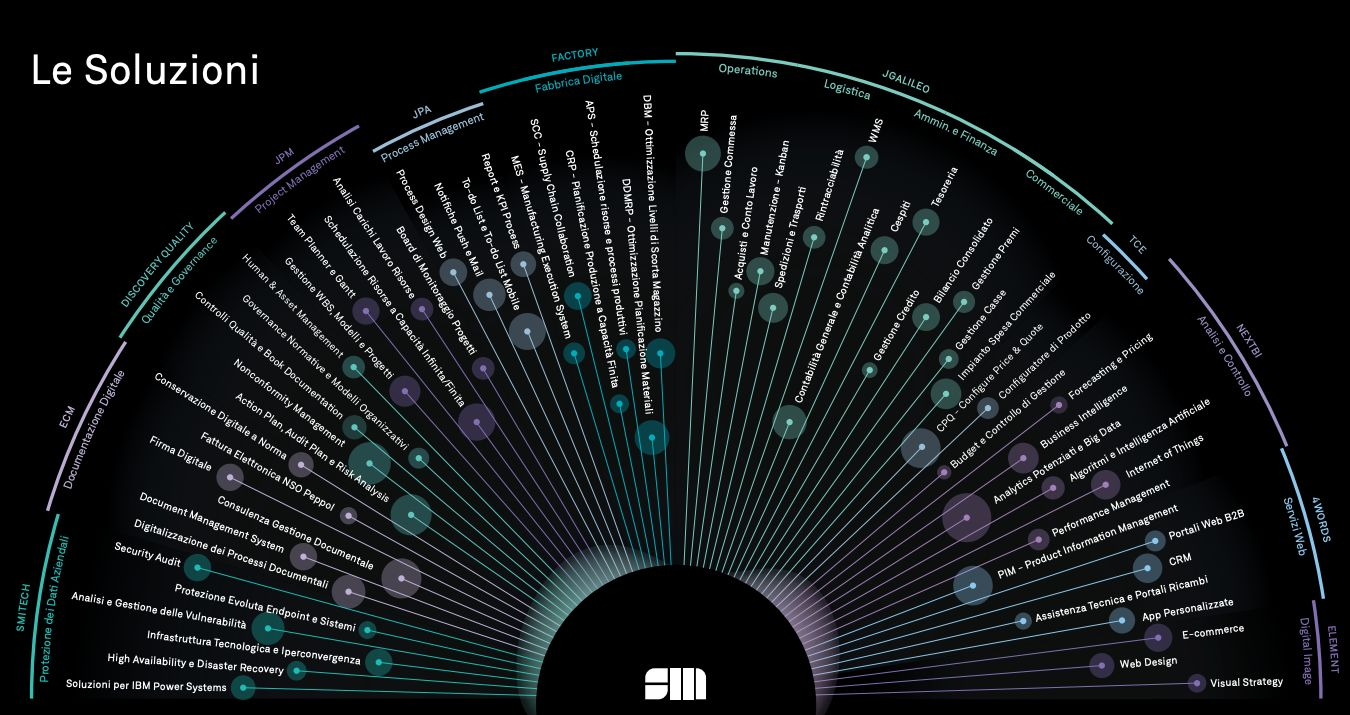
\includegraphics[width=1\columnwidth]{organizzazione-azienda} 
  \caption{Le BU di {\azienda} ed i loro prodotti}
  \label{fig:organizzazione-azienda}
\end{figure}

\newpage

\section{Il team di sviluppo}
Il team di sviluppo in cui ho lavorato fa parte della BU \textit{JPA} (\textit{Process Management}) e non si
occupa di sviluppare un prodotto specifico, ma ha come obiettivo quello di fornire supporto a tutti i team di sviluppo
dell'azienda. \\
L'azione di supporto si concretizza nella creazione di strumenti che permettano di automatizzare e semplificare
i processi di sviluppo, come ad esempio la compilazione, il rilascio di un prodotto o lo sviluppo di uno nuovo.
Il team si occupa anche dello sviluppo di un \textit{\gls{frameworkg}} interno che permette di creare applicazioni web
in modo semplice e veloce e di fornire supporto per la gestione di repository e di strumenti di \textit{\gls{continuous_integrationg}}

\section{Strumenti utilizzati}
I principali strumenti per lo sviluppo da me utilizzati sono stati i seguenti:\\
\begin{itemize}
  \item \textbf{Intellij IDEA:} un ambiente di sviluppo integrato (\gls{IDEg}) per il linguaggio di programmazione Java. Fornisce strumenti e funzionalità avanzate per supportare lo sviluppo efficiente del codice, il debug e la testing. Con la sua interfaccia user-friendly e le potenti funzionalità, come l'analisi statica del codice e il refactoring intelligente, IntelliJ IDEA è scelto da molti sviluppatori per creare applicazioni Java professionali;
  \item \textbf{WebStorm:} un IDE per lo sviluppo di applicazioni web, che fornisce un'esperienza di sviluppo ottimale. Grazie alla sua integrazione con strumenti di supporto per lo sviluppo web, come \textit{Node.js}, \textit{Angular}, \textit{React}, WebStorm permette di sviluppare applicazioni web moderne con facilità;
  \item \textbf{Neo4j Desktop:} un programma che permette di installare e gestire database \textit{Neo4j} in modo semplice e veloce. Permette di creare e gestire più database, di monitorare le performance e di eseguire query;
  \item \textbf{Git:} un sistema di controllo versione distribuito, utilizzato per il versionamento del codice sorgente; 
  \item \textbf{Gradle:} un sistema di automazione open source che gestisce le dipendenze e permette di automatizzare il processo di compilazione, testing, pubblicazione e deployment di un software;
  \item \textbf{Docker:} un progetto open source che automatizza il deployment di applicazioni all'interno di contenitori software, fornendo un'astrazione aggiuntiva grazie alla virtualizzazione a livello di sistema operativo di Linux;
  \item \textbf{Bitbucket:} un servizio di hosting per progetti che utilizzano Git come sistema di controllo versione. Fornisce strumenti per la collaborazione e la gestione del codice sorgente;
  \item \textbf{Jenkins:}  un software open source che permette di automatizzare il processo di \textit{build}, testing e deployment di un software;
  \item \textbf{Angular:} un {\gls{frameworkg}} open source per lo sviluppo di applicazioni web, scritto in TypeScript. 
  Fornisce un'architettura \gls{mvvm} e permette di creare applicazioni web dinamiche e scalabili;
  \item \textbf{Jira:} un software di tracciamento dei bug e gestione dei progetti, che permette di pianificare, monitorare e rilasciare software di qualità;
  \item \textbf{Confluence:} un software di collaborazione che permette di creare, organizzare e discutere documenti di progetto;
\end{itemize}

I linguaggi utilizzati sono i seguenti:\\

\begin{itemize}
  \item \textbf{Java:} un linguaggio di programmazione ad alto livello, orientato agli oggetti e a tipizzazione statica, che permette di creare applicazioni web, desktop e mobile;
  \item \textbf{Javascript:} un linguaggio di programmazione ad alto livello, orientato agli oggetti e a tipizzazione dinamica, che permette di creare applicazioni web dinamiche;
  \item \textbf{TypeScript:} un super-set di Javascript che permette di aggiungere tipizzazione statica al linguaggio;
  \item \textbf{Groovy:} un linguaggio di programmazione che permette di scrivere codice che viene eseguito sulla \gls{JVM};
  \item \textbf{Chyper:} un linguaggio di query dichiarativo per grafi, utilizzato per interrogare database \gls{Neo4j};
\end{itemize}
\newpage
\section{Rapporto con l'innovazione}

{\azienda} ha come obiettivo l’innovazione delle aziende clienti per contribuire al loro progresso, 
agevolando la trasformazione digitale ed è specializzata nella progettazione e nella realizzazione di soluzioni integrate, 
a supporto della riorganizzazione di tutti i processi aziendali e professionali.\\
Per raggiungere questo obiettivo, l'azienda indirizza ogni anno dal 15 al 20\% del proprio fatturato all’attività di Ricerca e Sviluppo.\\
Uno dei punti di forza di {\azienda} è la capacità di cogliere le idee e i suggerimenti dei clienti, dei dipendenti, dei collaboratori e trarne ispirazione per sviluppare nuovi prodotti e nuove soluzioni